\documentclass{article}

\usepackage[italian]{babel}
\usepackage[letterpaper,top=2cm,bottom=2cm,left=3cm,right=3cm,marginparwidth=1.75cm]{geometry}
\usepackage{amsmath}
\usepackage{graphicx}
\usepackage{subcaption}
\usepackage{textcomp}
\usepackage{float}
\usepackage{ragged2e}
\usepackage[dvipsnames]{xcolor}
\usepackage{fancyhdr}
\usepackage[colorlinks=true, allcolors=blue,
            pdfauthor={Matteo Drago},
            pdftitle={Bivacco 3 Fontane},
            pdfsubject={Diario bivacchi e trekking},
            pdfkeywords={bivacco, montagna, trekking, diario}]{hyperref}
                
\title{\textbf{Bivacco 3 Fontane - 1874 m s.l.m}}
\author{Matteo Drago}

% ==========================================================
% Impostazioni per il logo in ogni pagina
% ==========================================================
\pagestyle{fancy}
\fancyhf{} % Pulisce tutti i campi di intestazione e piè di pagina
\fancyhead[R]{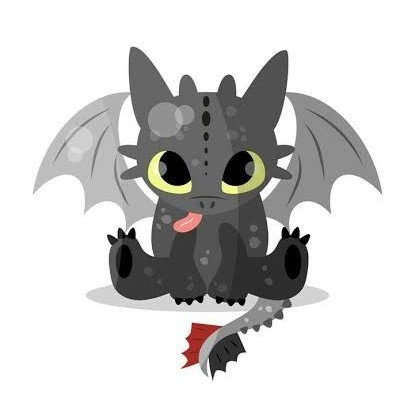
\includegraphics[height=1.5cm]{images/toothless.jpeg}} % Posiziona il logo a destra (R) nell'intestazione
\renewcommand{\headrulewidth}{0pt} % Rimuove la linea orizzontale nell'intestazione (opzionale)


\begin{document}
\maketitle
\thispagestyle{fancy} % Aggiungi questa riga

\begin{abstract}
Questo documento raccoglie e organizza le informazioni che ho acquisito nel corso degli anni sui bivacchi, basate sulle mie esperienze dirette. Sebbene non si proponga come una guida esaustiva e perfetta, offre il minimo indispensabile per una buona vita in bivacco, con consigli pratici e diretti per chiunque desideri affrontare al meglio queste pazze ma piacevoli avventure.
\end{abstract}

\section{Il bivacco}

% ==========================================================
% Immagine a sinistra, testo a destra allineato in alto
% ==========================================================
\noindent
\begin{minipage}[t]{0.45\textwidth}
  \vspace{0pt} % forza l'allineamento in alto
  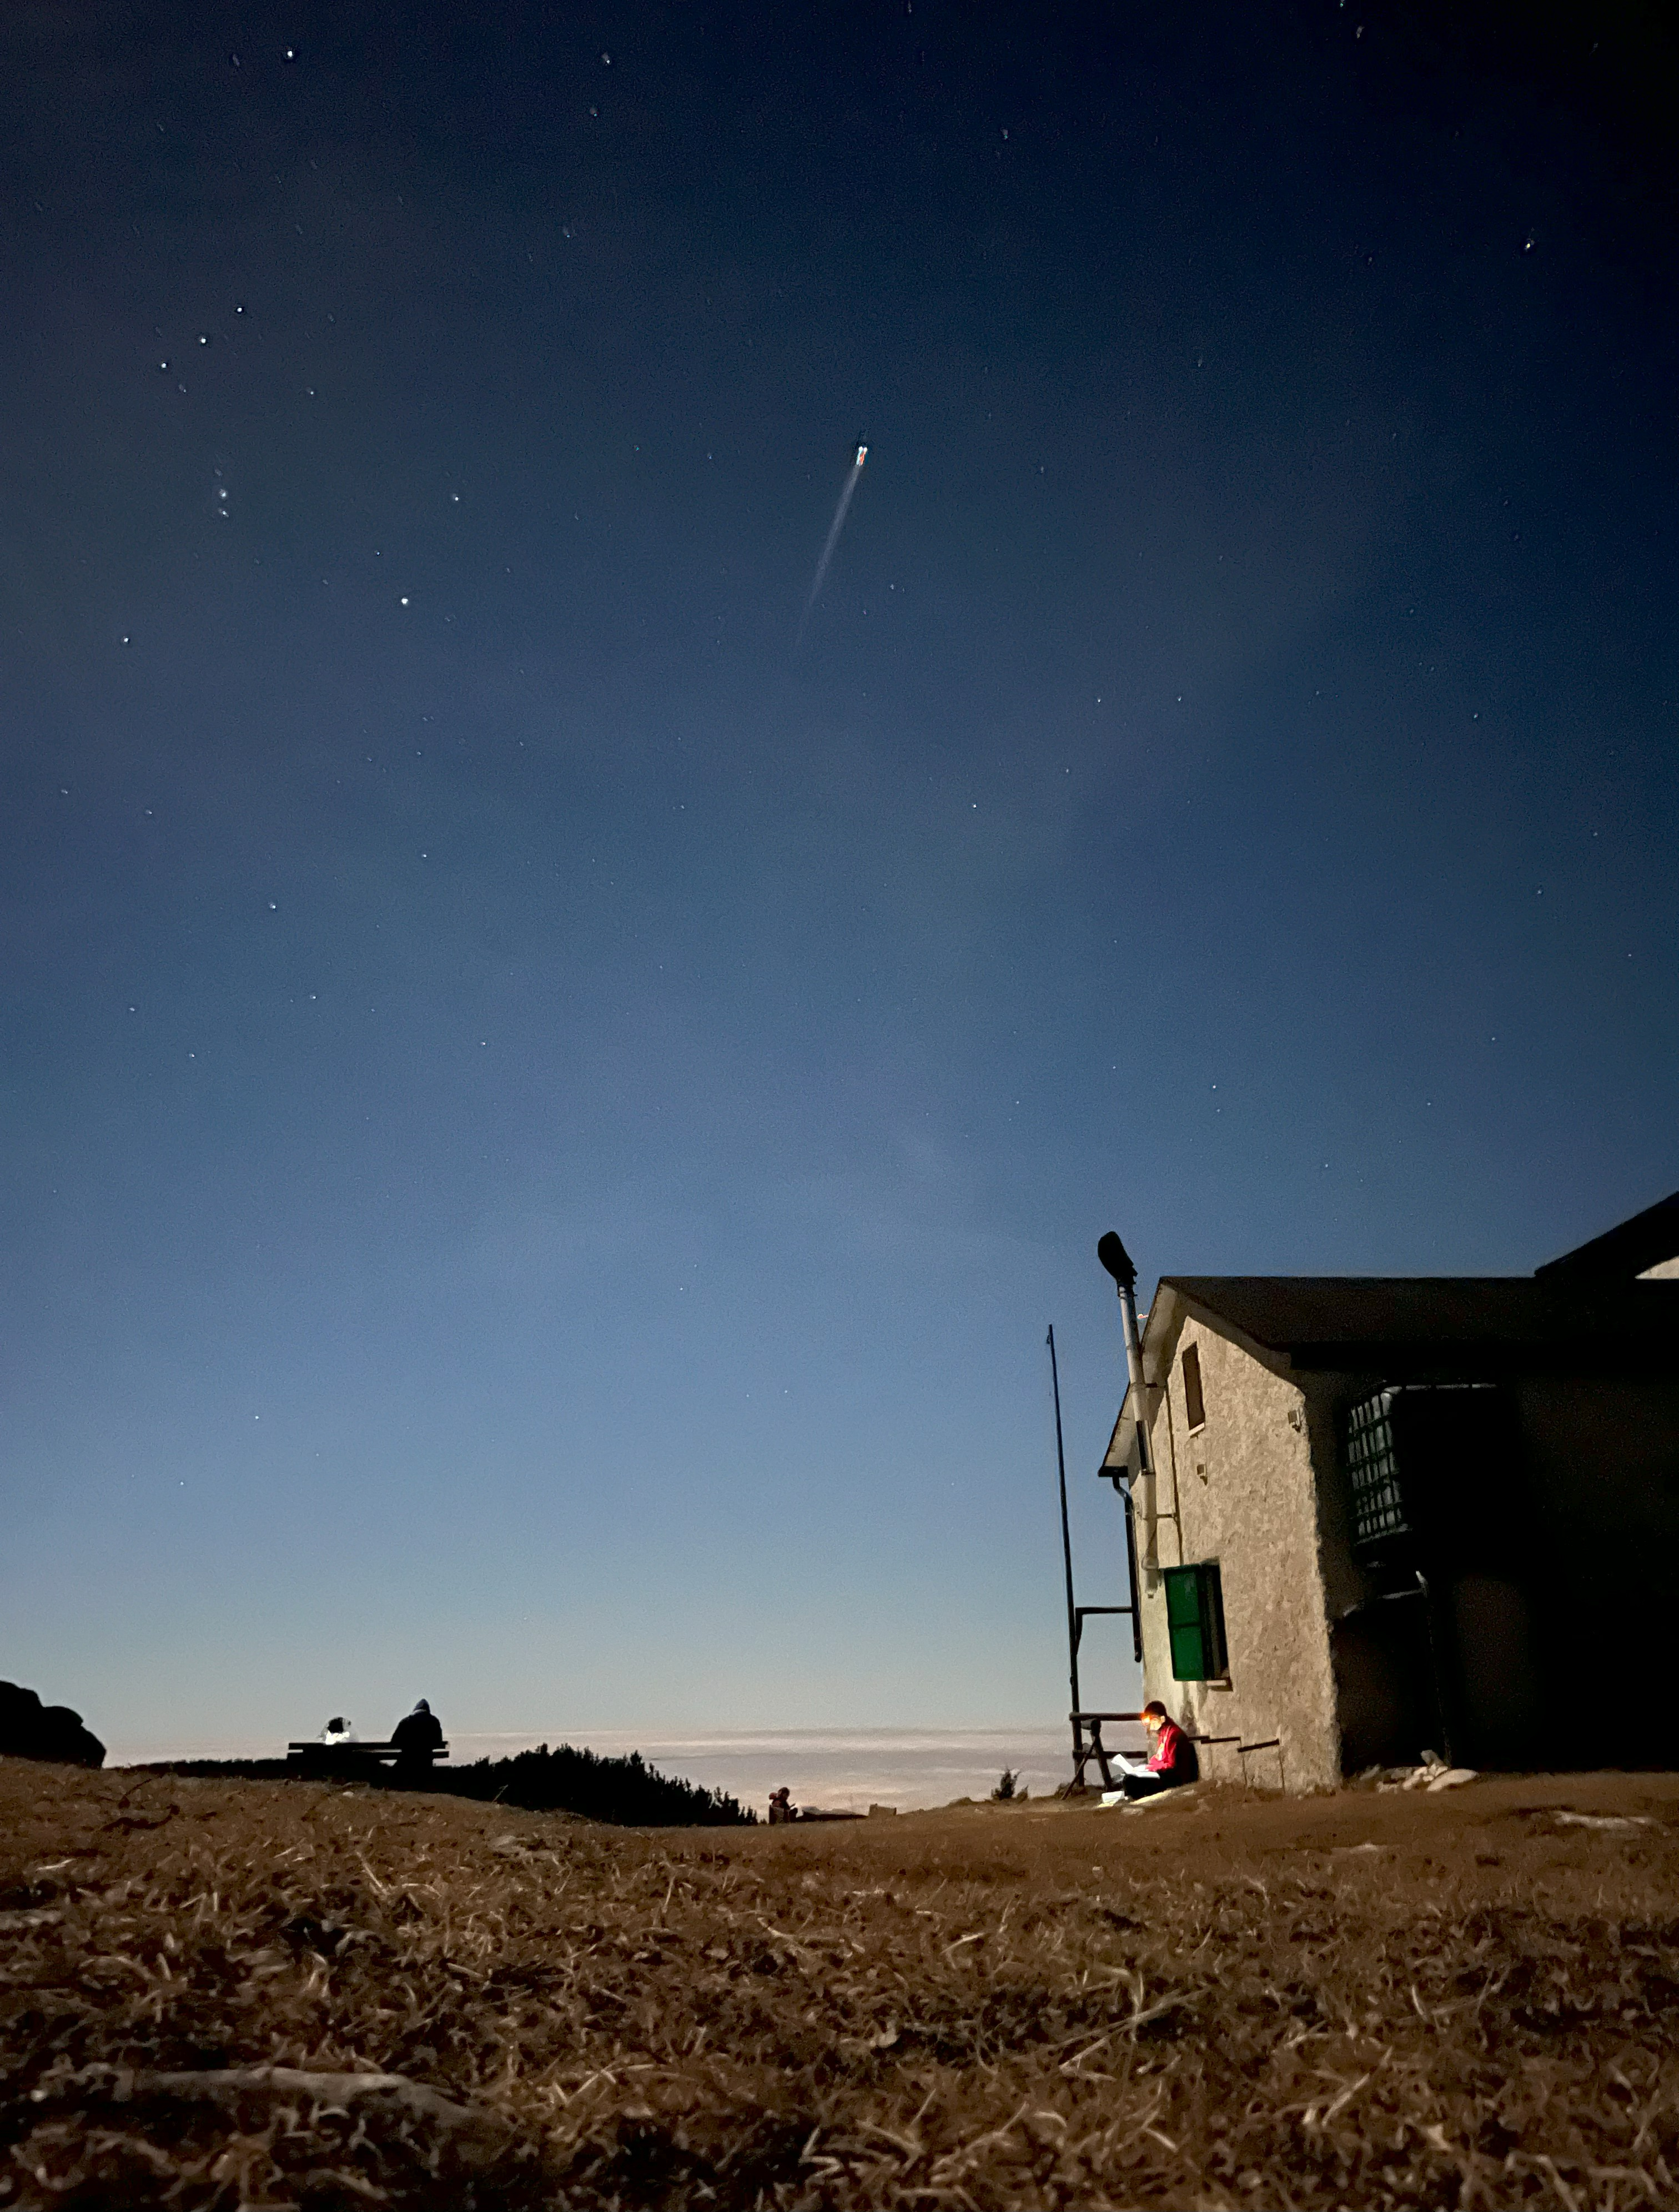
\includegraphics[width=\linewidth]{images/bivacco.jpg}
\end{minipage}%
\hfill
\begin{minipage}[t]{0.5\textwidth}
  \vspace{0pt} % forza l'allineamento in alto
  
  Gruppo montuoso\\
  \textbf{\large Altopiano dei 7 Comuni}
  \\[1em] % Aggiunge una riga vuota qui
  Località\\
  \textbf{\large Alta Val Galmarara}
  \\[1em] % Aggiunge una riga vuota qui
  Comune\\  
  \textbf{\large Lusiana (VI)}
  \\[1em] % Aggiunge una riga vuota qui
  Altezza\\  
  \textbf{\large 1874 m s.l.m.}
  \\[1em] % Aggiunge una riga vuota qui
  Apertura\\  
  \textbf{\large Gestito dagli Alpini di S. Caterina di Lusiana, sempre aperto}

\end{minipage}

\subsection{Caratteristiche}

La struttura è composta da due edifici adiacenti: uno, chiuso, di proprietà degli Alpini; l’altro, aperto, adibito a bivacco.  
\begin{itemize}
    \item \textbf{Piano terra}: due tavoli con sedie, una cucina economica, un lavello collegato a una cisterna esterna che raccoglie l’acqua piovana, una dispensa con vario materiale e un camino.
    \item \textbf{Piano superiore}: circa tre materassi in uno spazio ridotto, sufficiente ad accogliere 7–8 persone.
    \item \textbf{Spazio esterno}: curato dagli Alpini, con alcuni tavoli panoramici disposti all’aperto. 
\end{itemize}

Il bivacco in sé è piuttosto piccolo e offre lo stretto necessario per trascorrere una piacevole nottata.  

\textbf{\textcolor{OrangeRed}{Invito, tuttavia, a prestare molta attenzione al camino: il fumo fatica a uscire dalla canna fumaria, e durante la notte c'è la possibilità di dover arieggiare la stanza per non rimanere affumicati.}}

Nelle zone limitrofe non sono presenti fonti d’acqua (durante la salita se ne incontra una, ma in condizioni non ottimali). 

Il reperimento della legna non è semplice, data l’abbondanza di pino mugo; tuttavia, lungo il percorso di salita si trovano alcuni alberi utilizzabili.


\section{Come ci siamo arrivati}
Il bivacco è stato inserito in un giro di due giorni che comprendeva il Bivacco 3 Fontane e il Bivacco Casera Trentin.

Abbiamo parcheggiato l’auto al bivio di Basa Senocio (1100 m s.l.m.) e da lì ci siamo incamminati. Dopo una pausa pranzo presso Malga Galmarara, abbiamo proseguito fino a raggiungere il Bivacco 3 Fontane. Il giorno successivo siamo ripartiti in direzione del Bivacco Casera Trentin.


\begin{figure}[htbp!]
    \centering
    % Colonna di sinistra, allineata in alto
    \begin{subfigure}[t]{0.45\textwidth}
        \centering
        \vspace{0pt} % Forziamo l'allineamento in alto
        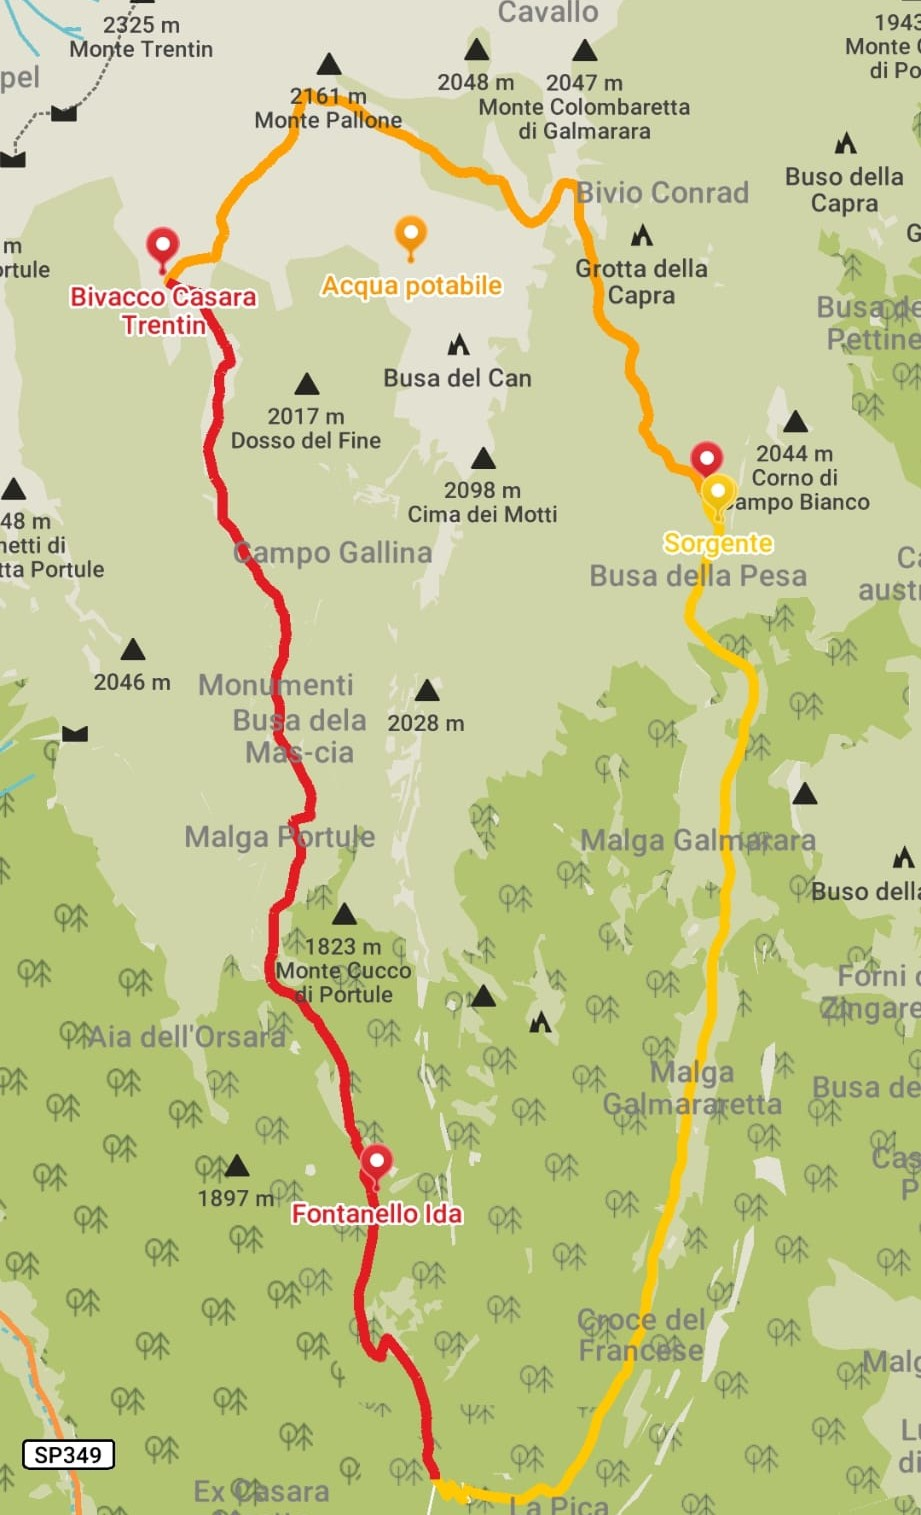
\includegraphics[width=\textwidth]{images/sentiero_mapsMe.jpg}
        \caption{Sentiero su Maps.Me.}
        \label{fig:foto_lunga}
    \end{subfigure}
    \hfill
    % Colonna di destra, allineata in alto
    \begin{subfigure}[t]{0.45\textwidth}
        \centering
        \vspace{0pt} % Forziamo l'allineamento in alto anche qui
        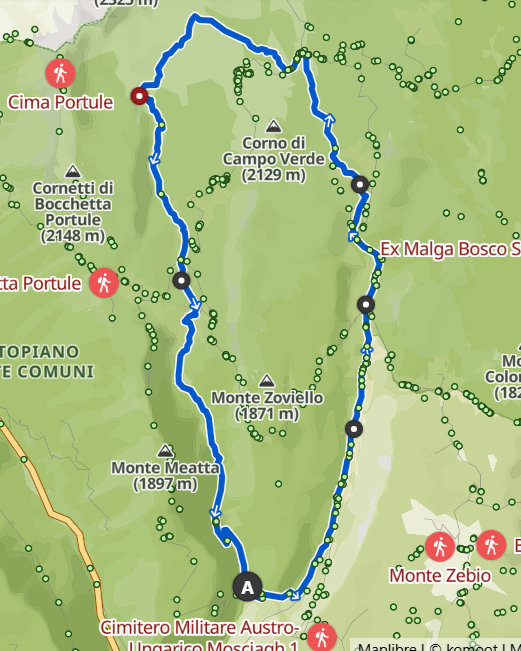
\includegraphics[width=\textwidth]{images/sentiero_komoot.png}
        \caption{Sentiero su Komoot.}
        \label{fig:foto_corta1}
        \vspace{1em} % Aggiunge un po' di spazio tra le due foto
        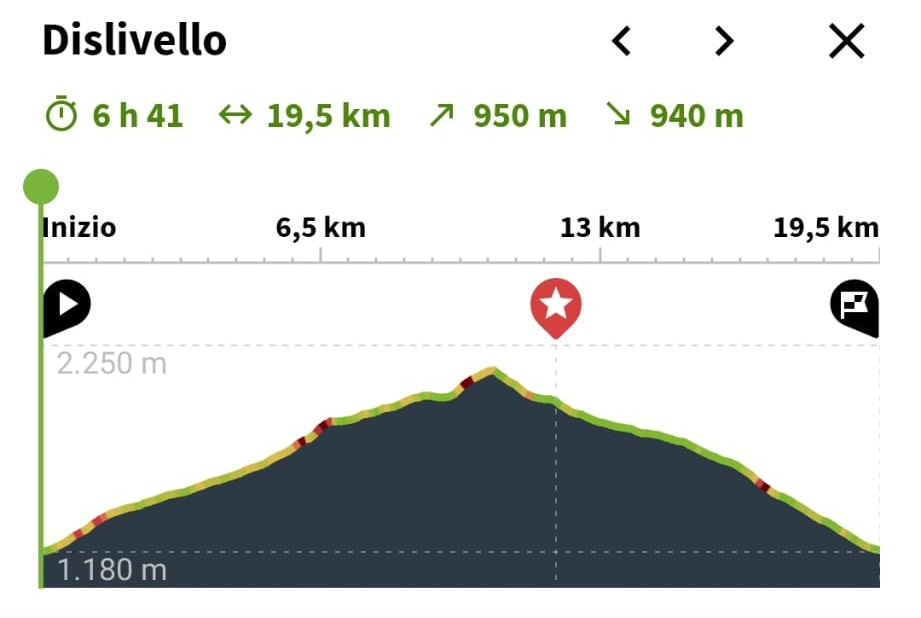
\includegraphics[width=\textwidth]{images/profilo_altimetrico.jpg}
        \caption{Profilo altimetrico del percorso.}
        \label{fig:foto_corta2}
    \end{subfigure}
    % Didascalia generale per l'intera figura
    \caption{Il sentiero e i dettagli del percorso.}
    \label{fig:panoramica_dettagli}
\end{figure}


\section{Non ti scordar di me}
\textbf{\textcolor{BurntOrange}{Ricorda: il bivacco è un bene comune. Il suo futuro dipende dal rispetto e dal senso civico dei visitatori. Usalo con cura e lascialo più pulito di come l'hai trovato.}}


\section{Esperienza personale}
Si è trattata di un'esperienza di 3 giorni con l'obiettivo di pernottare in 2 bivacchi, il 3 Fontane e la Casera Trentin. 
Il percorso per arrivare non è stato difficile, la neve non era molto profonda anche se fatto a dicembre.
Il primo bivacco si è dimostrato panoramico ma all'interno molto piccolo tantè che per risparmiare spazio ho dormito all'interno in amaca. Inoltre, il camino durante la notte si è dimostrato pessimo: il fumo anzichè uscire dal camino entrava tutto all'interno e per questo motivo abbiamo dovuto far notte ad arieggiare il bivacco nella speranza di non cuocerci. Il giorno dopo siamo poi partiti con meta la Casera Trentin.


\section{Alcune foto}

% Sezione Alcune foto

\begin{figure}[htbp!]
    \centering
    % Prima riga: Due foto (QUESTA È LA PRIMA FIGURA)
    \begin{subfigure}[b]{0.45\textwidth}
        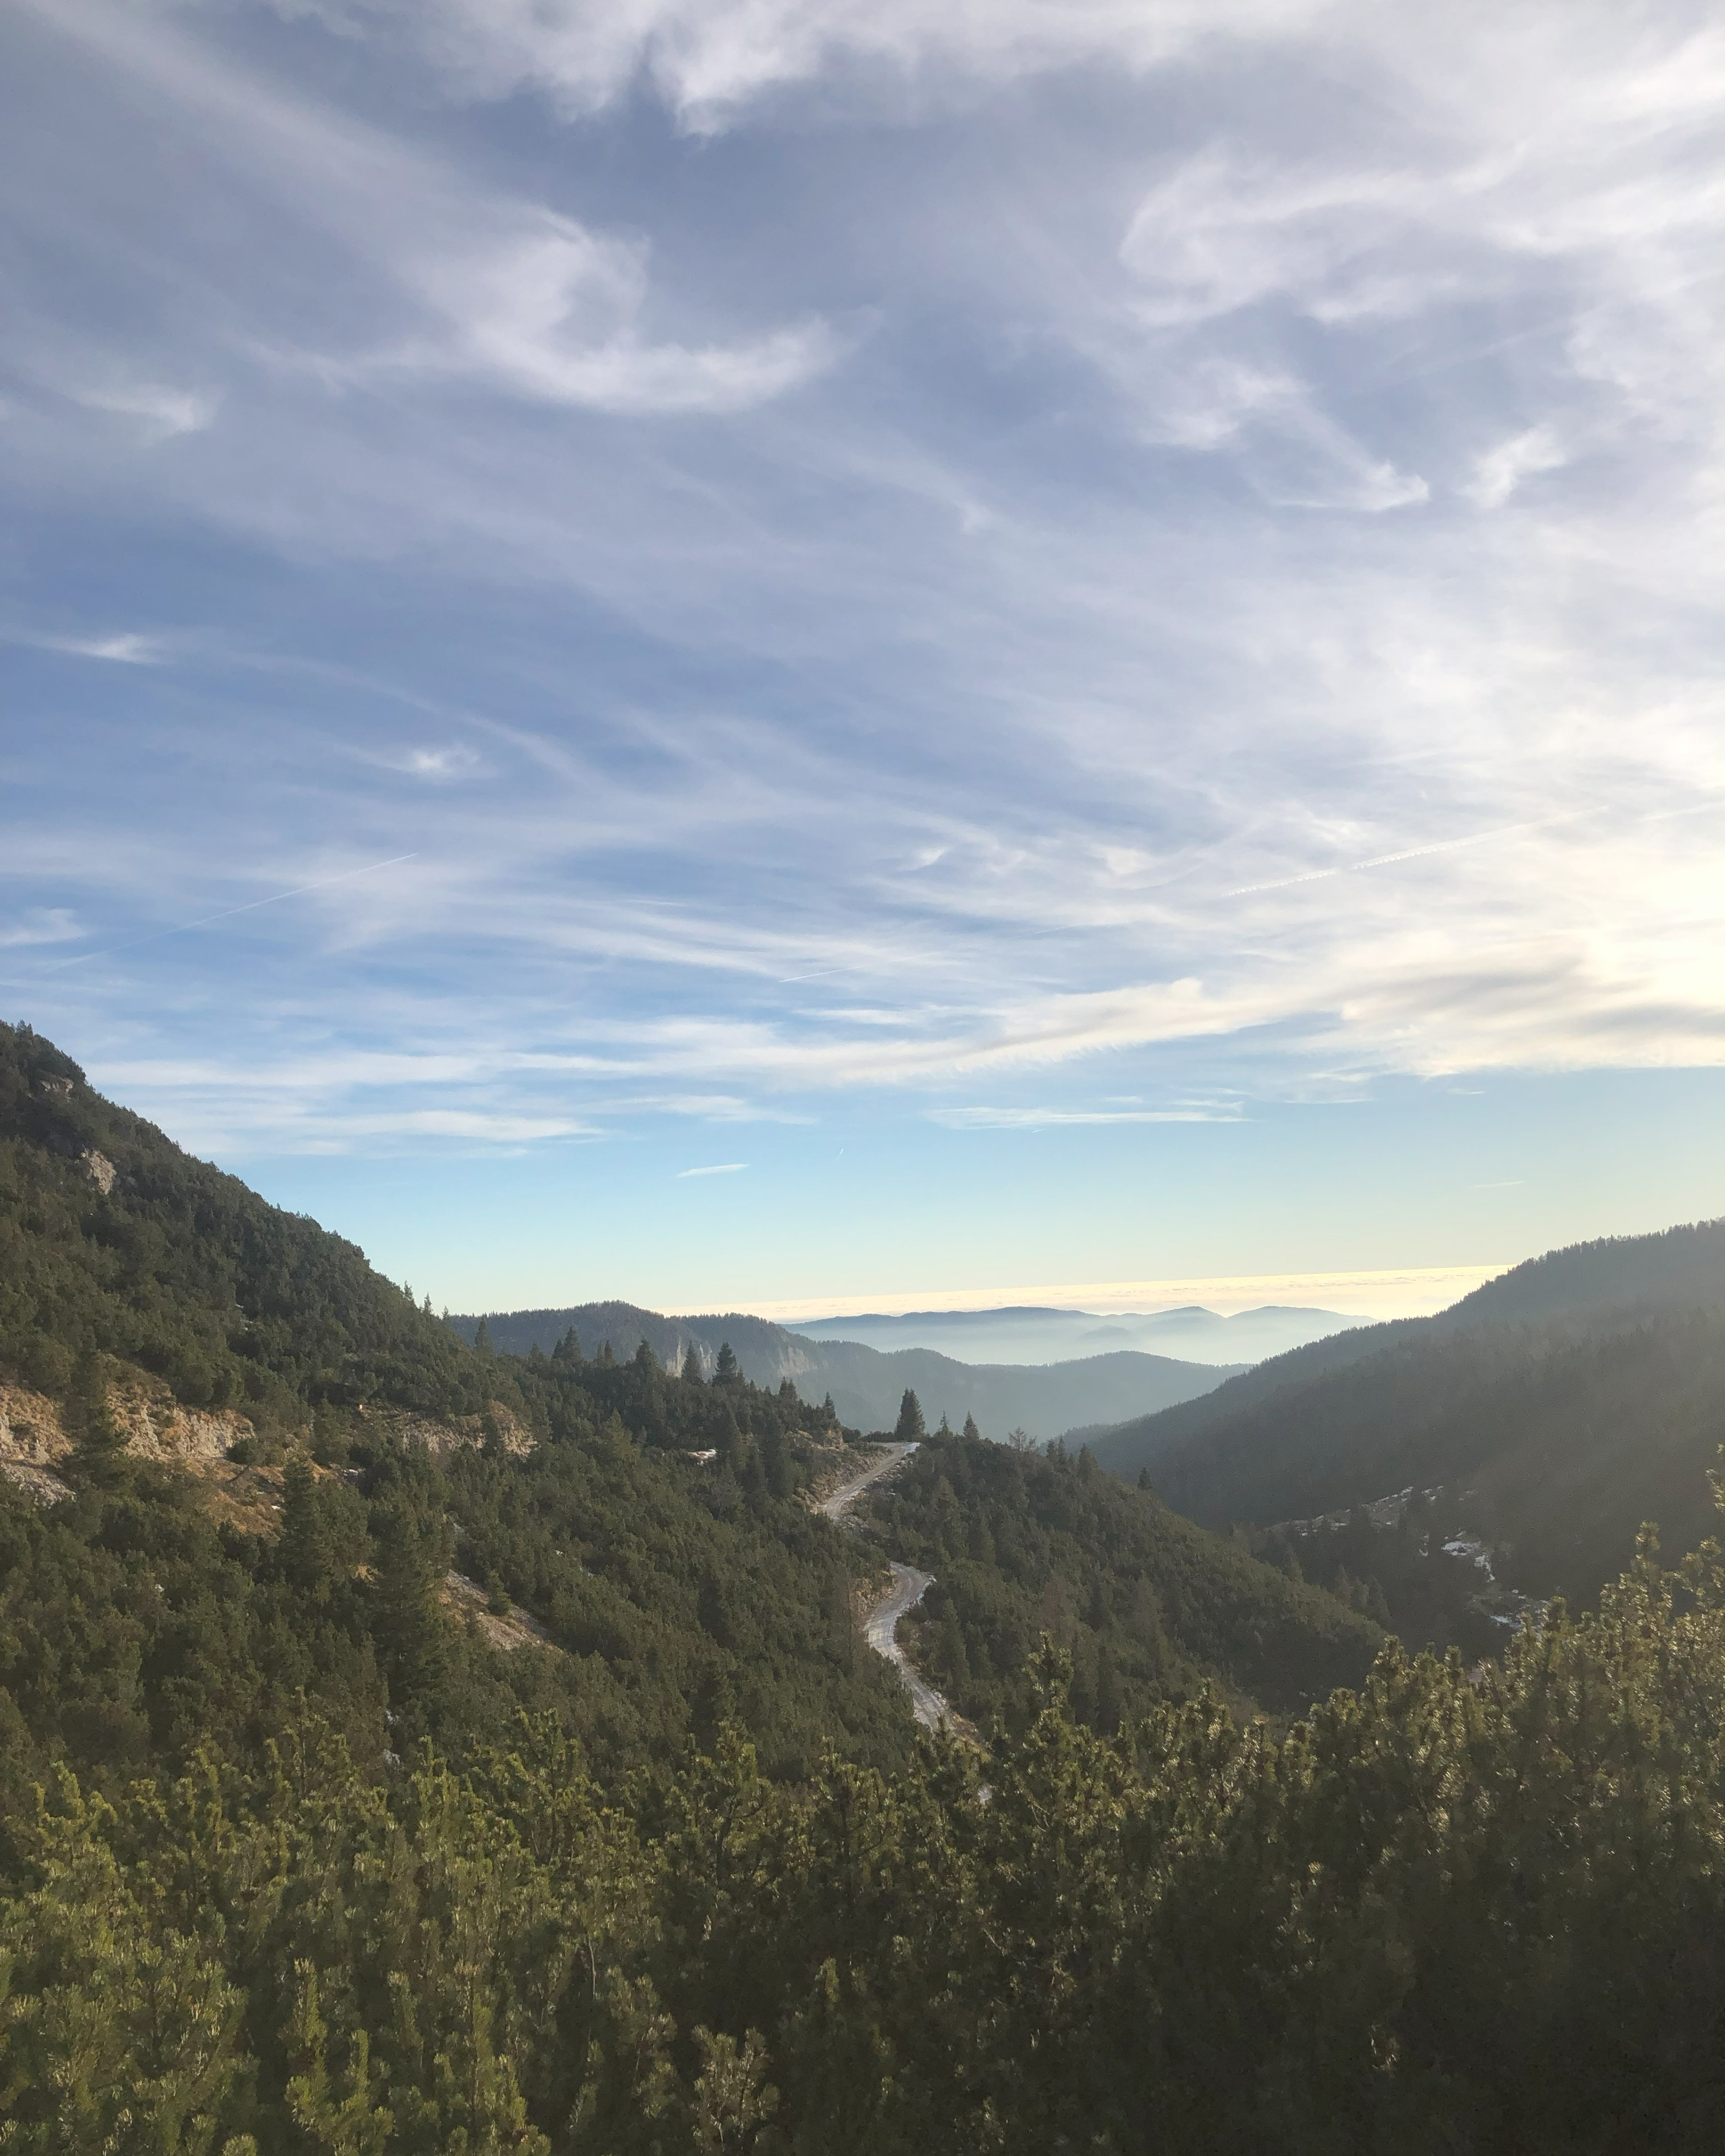
\includegraphics[width=\textwidth]{images/foto_sentiero.jpg}
        \caption{Sentiero.}
    \end{subfigure}
    \hfill
    \begin{subfigure}[b]{0.45\textwidth}
        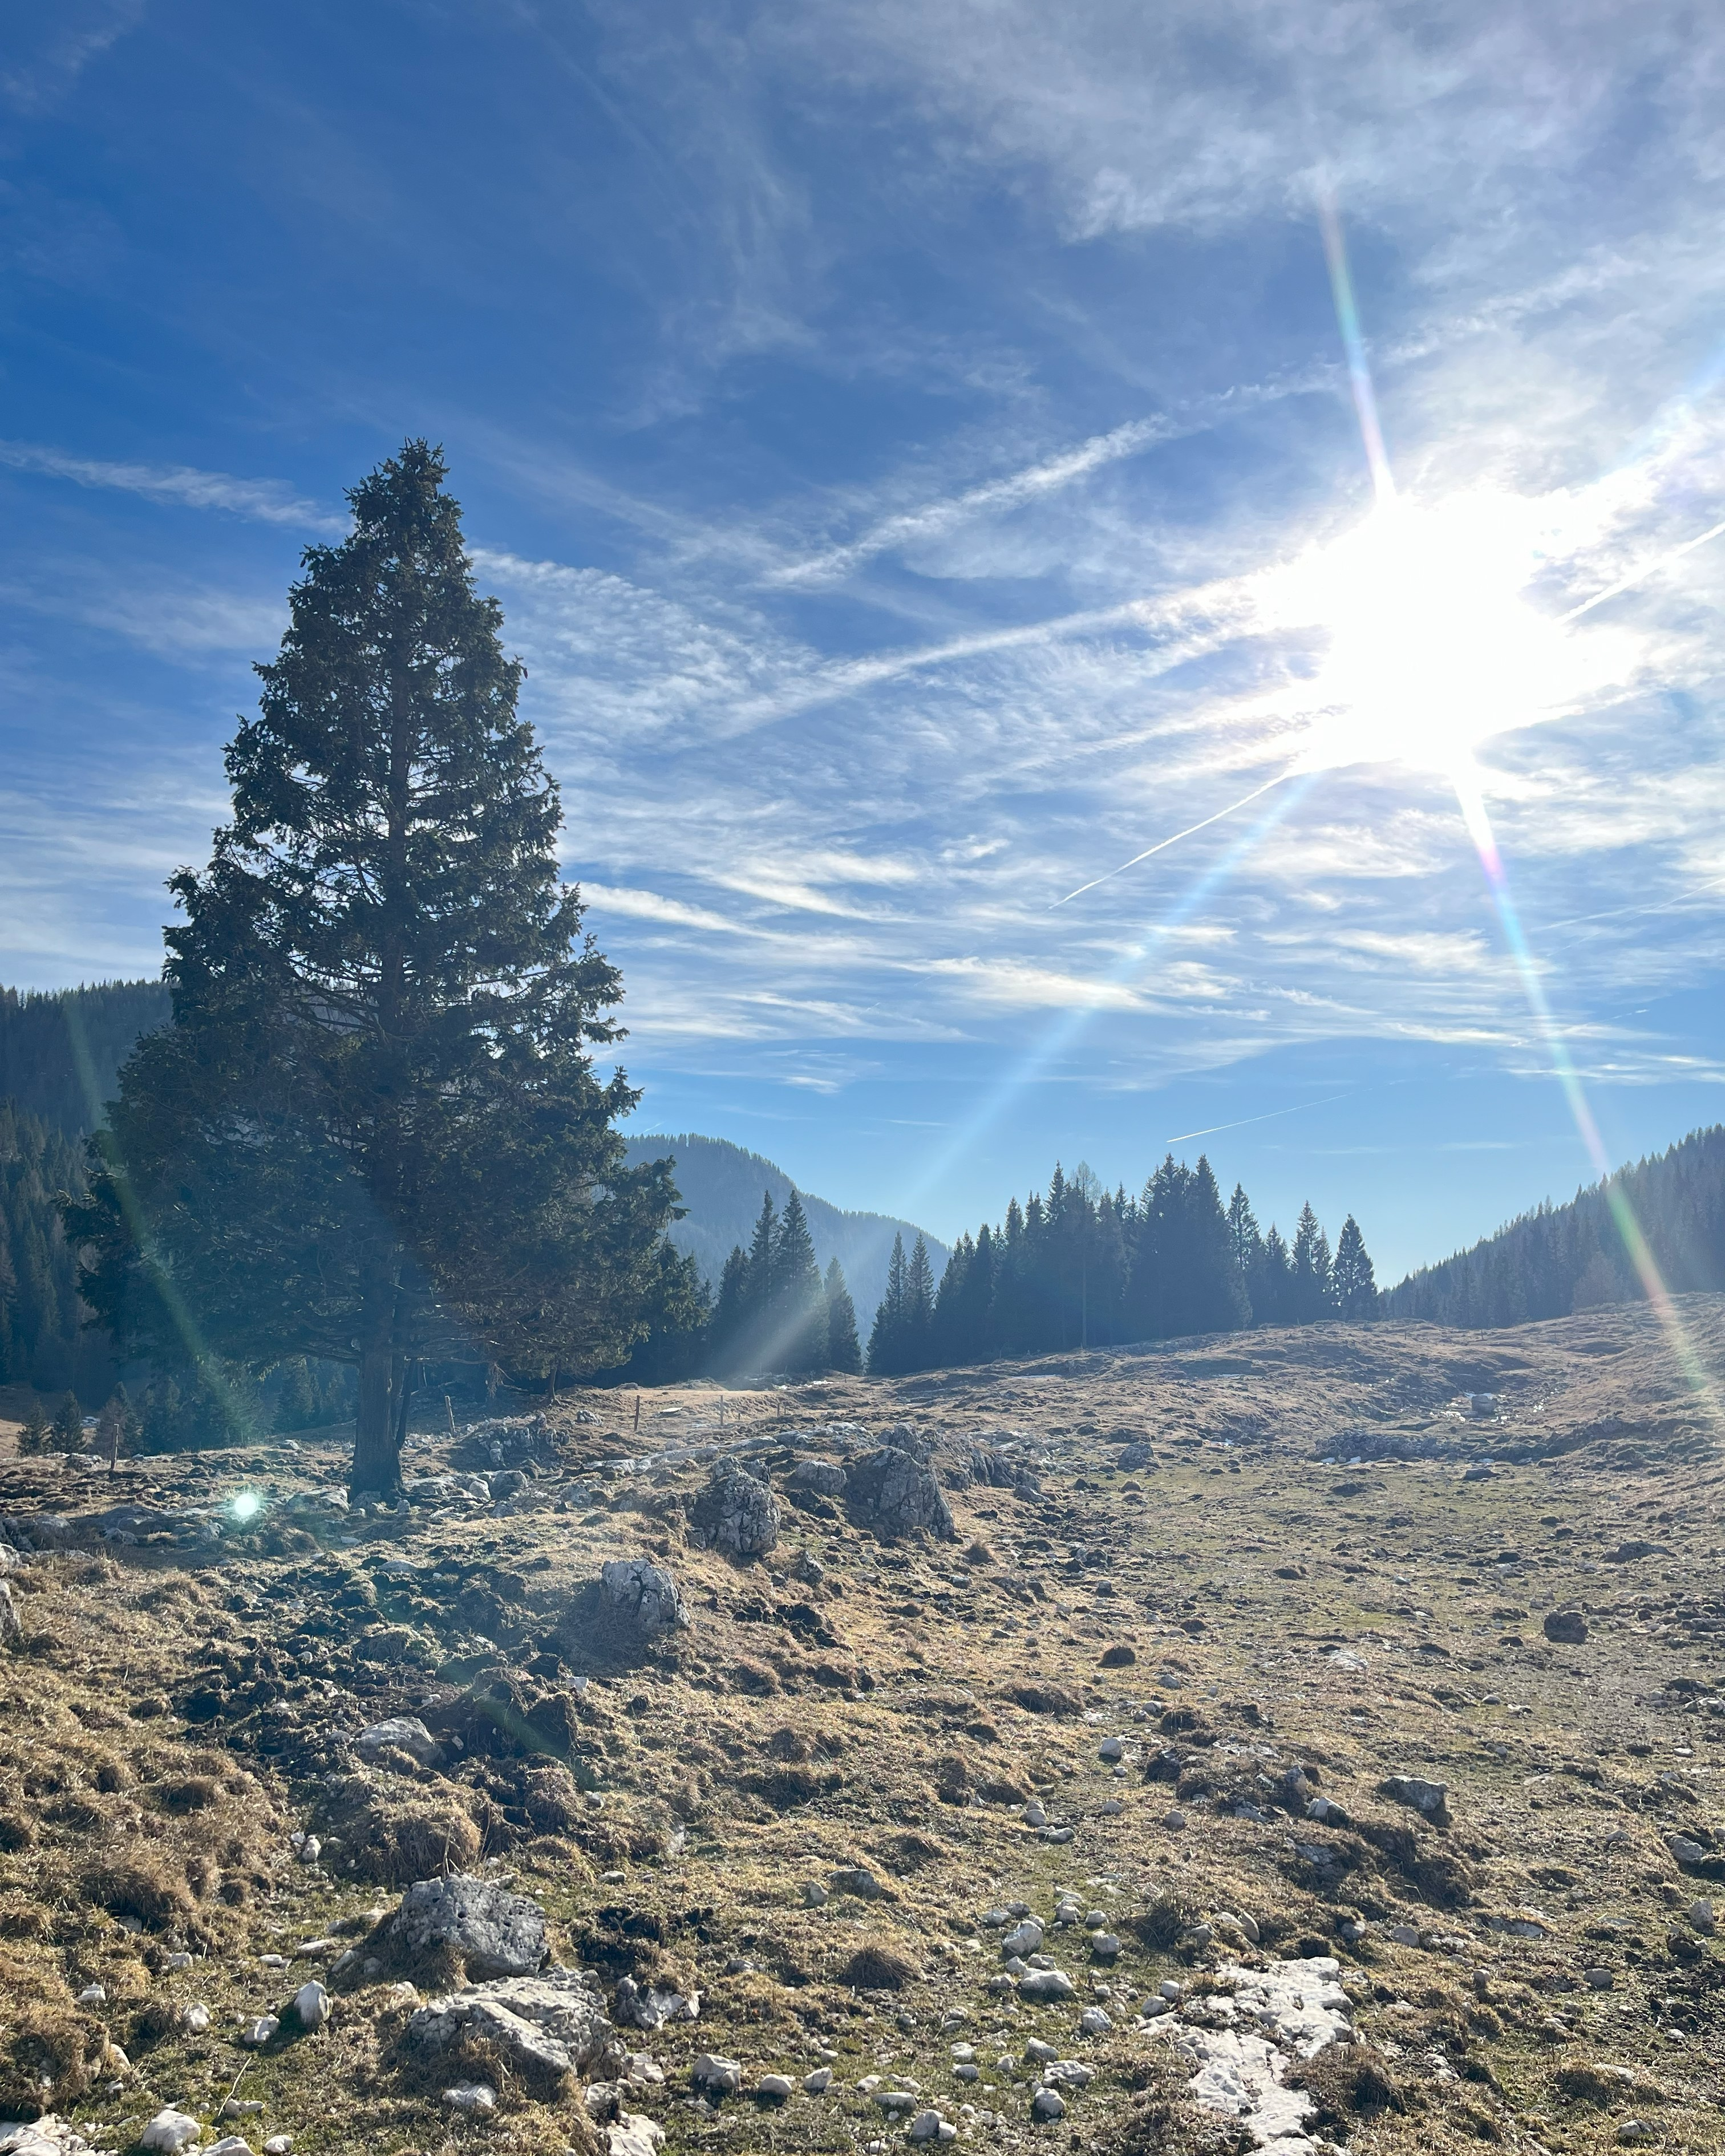
\includegraphics[width=\textwidth]{images/foto_paesaggio.jpg}
        \caption{Paesaggio.}
    \end{subfigure}

    \caption{Alcune foto.}
\end{figure}


\begin{figure}[H]
    \centering
    % Seconda riga: Tre foto (QUESTA È LA SECONDA FIGURA)
    \begin{subfigure}[b]{0.45\textwidth}
        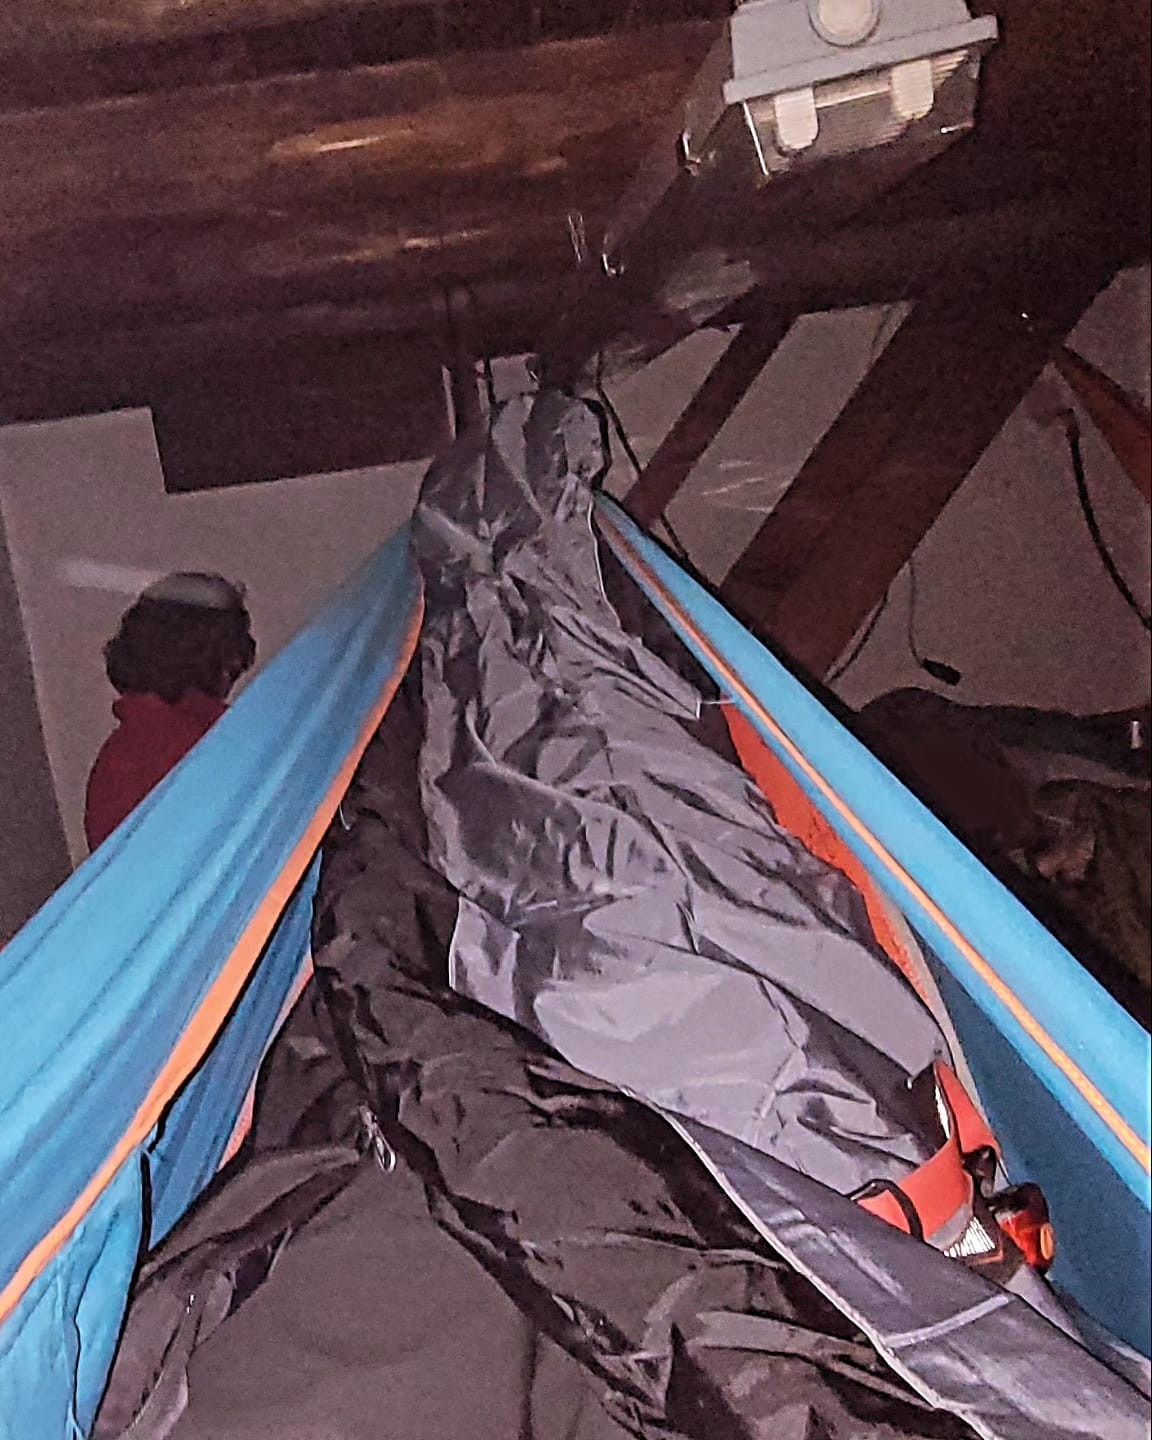
\includegraphics[width=\textwidth]{images/foto_amaca.jpg}
        \caption{Notte in amaca.}
    \end{subfigure}
    \hfill
    \begin{subfigure}[b]{0.45\textwidth}
        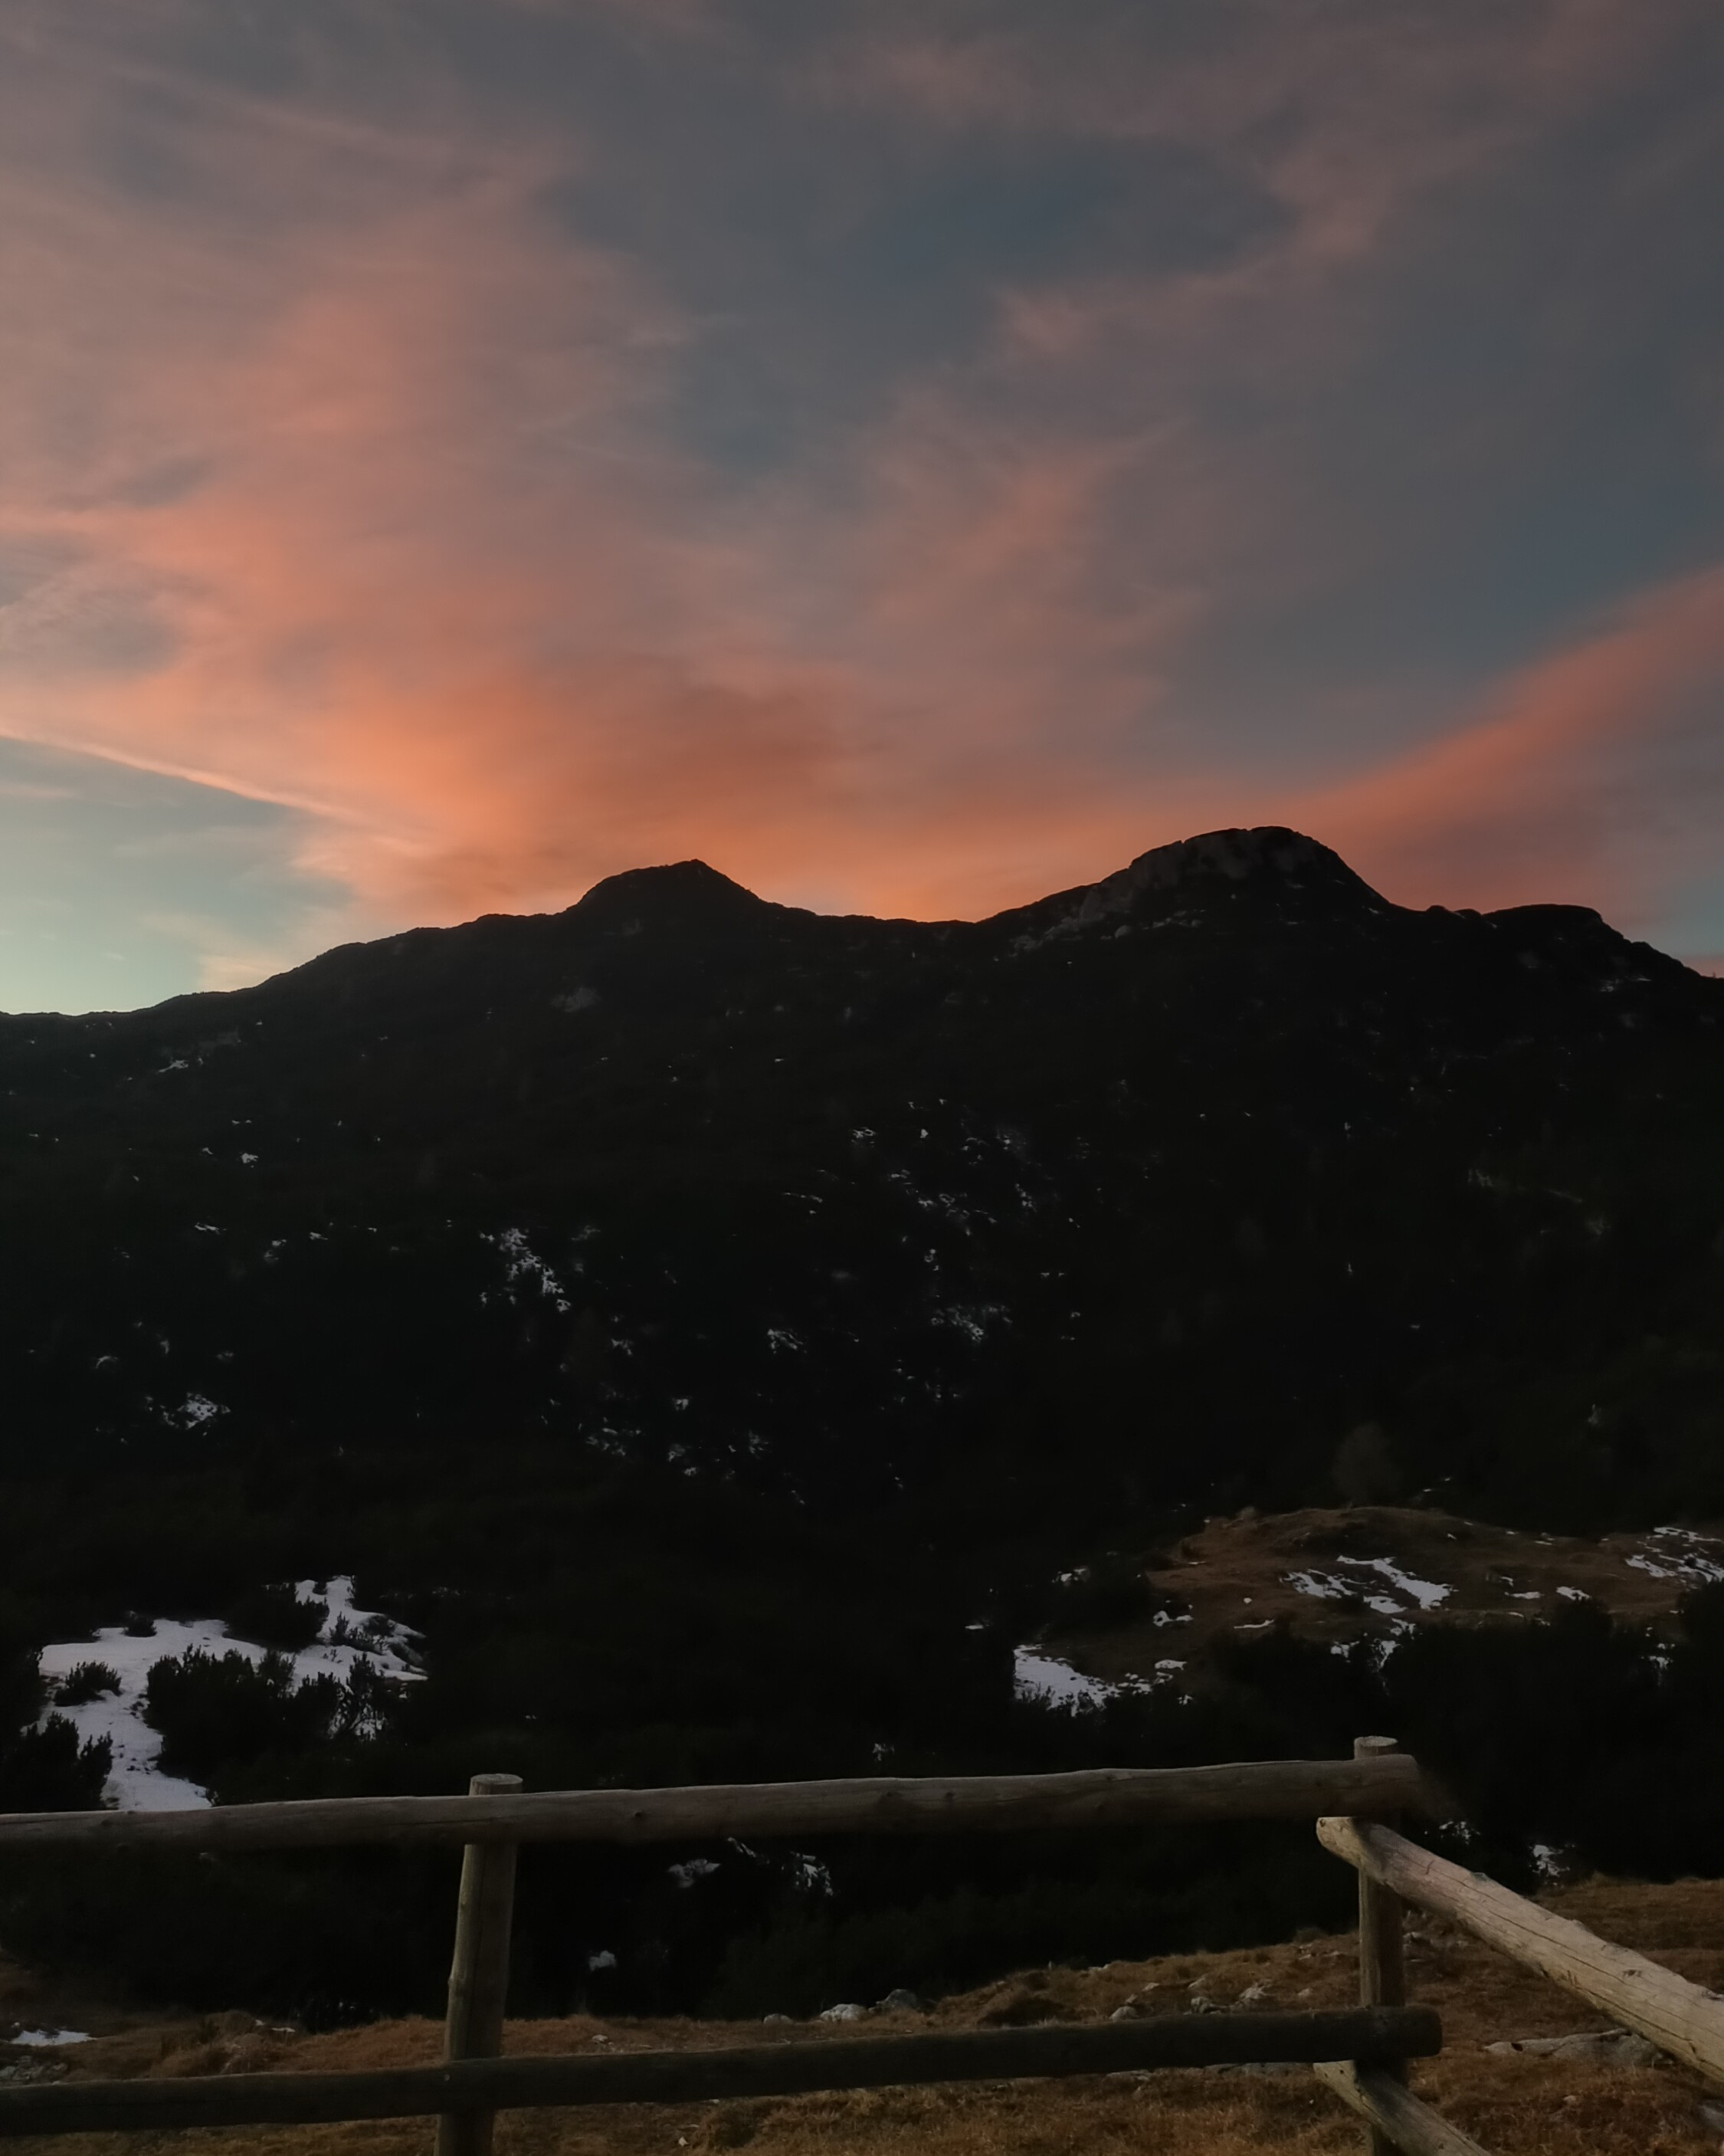
\includegraphics[width=\textwidth]{images/foto_notte.jpg}
        \caption{Vista di notte.}
    \end{subfigure}
    \hfill

    \caption{Selezione di fotografie del percorso e della vista dal bivacco.}
\end{figure}

\end{document}
